\documentclass{sig-alternate-10pt}
\newcommand\correspondingauthor{\thanks{Corresponding Author}}
\usepackage[paperwidth=8.5in, paperheight=11in, margin=1in]{geometry}
\usepackage{graphicx,url} 
\usepackage[utf8]{inputenc} 
\usepackage{graphicx} 
%\usepackage{caption}
\graphicspath{{img/}}
\usepackage [autostyle, english = american]{csquotes}
\MakeOuterQuote{"}
\usepackage{array, makecell}
\setcellgapes{4pt}
\usepackage[T1]{fontenc}
\usepackage{verbatim}
\usepackage{color}
\usepackage{multirow}

\definecolor{acolor}{rgb}{1,0.5,0}
%\newcommand{\dg}{\color{acolor}}
%\newcommand{\al}{\color{red}}
%\newcommand{\rc}{\color{blue}}

% Para retirar as cores do PDF, basta comentar os três comandos acima e descomentar os abaixo:

\newcommand{\dg}{}
\newcommand{\al}{}
\newcommand{\rc}{}

\title{A Brief Survey on Cloud Database Consistency}

\def\sharedaffiliation{%
\end{tabular}
\begin{tabular}{c}}
%
\begin{document}
	\pagestyle{empty}
	
	\numberofauthors{3}
	\author{
		% 1st. author
		\alignauthor 
        Robson A. Campêlo\correspondingauthor 
		% 2nd. author
		\alignauthor 
        Dorgival Guedes     
		% 3rd. author
		\alignauthor 
        Alberto H. F. Laender    
		\sharedaffiliation
		\affaddr{Department of Computer Science}  \\
		\affaddr{Universidade Federal de Minas Gerais}   \\
		\affaddr{Belo Horizonte, MG, Brazil} \\
		\email{\{robson.campelo, dorgival, laender\}@dcc.ufmg.br}
	}

\maketitle

\begin{abstract}
Cloud computing is a general term that involves delivering hosted services over the Internet. With the accelerated growth in the volume of data used by applications, several organizations have moved their data into cloud servers to provide scalable, reliable and highly available services. A particularly challenging issue that arises in the context of cloud storage systems with geo\-graphi\-cally-distributed data replication is how to reach a consistent state for all replicas. In this survey, we review major aspects related to consistency issues in cloud data storage systems, categorizing recently proposed methods into three catego\-ries: (1)~static consistency methods, (2) dynamic consistency methods, and (3) consistency monitoring methods. 
\end{abstract}
\\

\section{Introduction}

%Cloud computing is a general term that involves delivering hosted services over the Internet. The term ``cloud'' is an abstraction of this new model that arose from a network connectivity architecture involving several {\al data} providers stored in external servers.

Cloud computing is a general term that includes the idea of delivering hosted services over the Internet. The term ``cloud'' is an abstraction of this new model that arose from a common representation of a network, since the particular location of a service is not relevant, {\al which means that services and data providers are seen} as existing ``in the network cloud''.

In recent years, cloud computing has emerged as a paradigm that attracts the interest of organizations and users {\al due to} its potential for cost savings, unlimited scalability and elasticity in data management. In this paradigm, users acquire computing and storage resources in a pricing model which is known as \emph{pay-as-you-go} \cite{Al-Roomi13}. According to this model, IT resources are offered in an unlimited way and the payment is made according to the actual resources used for a certain period, similarly to the traditional energy pricing model.


%Cloud deployment models can be grouped into four types: private, public, hybrid and community~\cite{mell2009nist}. In these environments, the services are provided without the users' concern about how this process occurs. 
Depending on the kind of resource offered to the users, cloud services tend be grouped in the following three basic models: \emph{Software as a Service} (SaaS)~\cite{dubey2007delivering}, \emph{Platform as a Service} (PaaS)~\cite{beimborn2011platform} and \emph{Infrastructure as a Service} (IaaS)~\cite{bhardwaj2010cloud}. As an extension of this classi\-fication, when the service refers to a database, the model is known as \emph{Database as a Service} (DBaaS)~\cite{curino2011relational}, {\al which is the focus of this survey}. {\rc  This model provides transparent mechanisms to create, store, access and update databases. Moreover, the database service provider ensures full responsibility for the database administration, guaranteeing backup, reorganization and migration to new system versions.}
%Moreover, the database service provider ensures the entire responsibility of  database adaministration, i.e., database backup, administration, reorganization or migration from one database version without impacting such an organization.

%With the accelerated growth in the volume of data {\al used} by the applications, several organizations have moved their data into cloud servers to provide scalable, reliable and highly available services. Cloud servers enable service providers to store and customize their data across multiple data centers, separating them physically to meet a growing demand. In this way, services can replicate their state among geographically diverse locations and direct the user to the nearest or most recently accessed one. %location. 
%Thus, replication has become an essential feature of this storage model and is extensively exploited in cloud environments \cite{Chang06bigtable:a, Ibrahim12}. Moreover, replication allows users to obtain various features such as fast access, improved performance and high availability.
%
% DG: o parágrafo acima foi reorganizado na forma a seguir:
%
The use of DBaaS cloud servers enables service providers to replicate
and customize their data over multiple servers, which can be physically separated and placed in different data centers.
By doing so, {\al they} can meet a growing demand by directing users to the nearest, or most recently accessed server. In that way, replication allows {\al them} to achieve features such as fast access,improved performance and higher availability. Thus, replication has become an essential feature of this storage model and is extensively exploited in cloud environments~\cite{Chang06bigtable:a, Ibrahim12}.

A particularly challenging issue that arises in the context of cloud storage systems with geo\-graphi\-cal\-ly-distributed data replication is how to reach a consistent state in all replicas. {\dg In the cloud environment, computer failures and network partitions cannot be completely avoided.} Enforcing synchronous replication to ensure strong consistency {\dg in such an environment} incurs in a significant performance overhead, due to the problem of high network latency between data centers~\cite{goel2007data} 
{\dg and the fact that network partitions may lead to service unavailability~\cite{Brewer2000}}. 
As a consequence, specific models have been proposed to ensure weaker or relaxed consistency guarantees.
%in the form of {\bf eventual consistency.}

Several cloud storage services choose to ensure availability and performance {\dg even in the presence of network partitions} rather than {\al to use} a stronger consistency model. NoSQL-based data storage environments provide consistency properties in  eventual mode~\cite{Vogels:2009}. However, using this type of consistency increases the probability of reading obsolete data, {\al since} the replicas being accessed may not have received the most recent writes. This led to the development of adaptive consistency solutions, which were introduced to allow adjusting the level of consistency at runtime in order to improve performance or reduce costs, while maintaining the percentage of obsolete reads at low levels~\cite{chihoub2012harmony, esteves2012quality, Terry:2013}.

A consistency model in distributed environments seeks to guarantee the consistency of an update operation, as well as the access to an updated object. Obtaining the correct balance between consistency and availability is one of the challenges still existing in cloud computing~\cite{Elbushra:2014}. In this survey, we focus on state-of-the-art  methods for data consistency in cloud environments. Considering the different solutions, we categorize these recently proposed methods into three %potential 
distinct categories: (1) static consistency methods, (2) dynamic consistency methods and (3) consistency monitoring methods.

The remainder of this survey is organized as follows. In Section 2, we present general concepts related to cloud database management. In Section 3, we approach the main consistency models adopted by existing distributed storage systems. 
%In Sections 4 and 5, respectively, we present a taxonomy proposed to categorize the {\al  most prominent} consistency methods {\al found in the literature} and overview {\al each one} of them.
In Sections 4 and 5, we present, respectively, a taxonomy proposed to categorize the most prominent consistency methods found in the literature and an overview~of the main approaches adopted to implement them. In Section~6, we provide a sum-up discussion emphasizing the main aspects of the surveyed methods.
%we discuss the methods} we have surveyed. 
Finally, in Section 7, we conclude the survey by summarizing its major issues.
%\\
\vspace{2mm}

\section{Cloud Database Management}
\label{sec:clouddbmngmt}
In this section, we present general concepts related to cloud database management in order to provide a better understanding of the key issues that affect data consistency. Initially, we approach the architectural aspects of the DBaaS model. After that, we highlight the cloud storage infrastructure requirements and describe the ACID properties. Finally, we introduce the CAP theorem and discuss its associated trade-offs. 
\vspace{1mm}

\subsection{Architectural Aspects of the DBaaS \\ Model}

In the DBaaS model, the architecture is often distributed and data can be stored in possibly hundreds of machines, where the resources are shared among the clients~\cite{Xiong:2011}. As previously mentioned, one of the techniques used to obtain %various 
{\al specific} features
such as fast access, improved performance and high availability is to replicate data in geographically distinct locations.  % Hence, replication is an essential resource in the DBaaS model. % Repetido da introdução

{\al For example, in a scenario in which a failure occurs} in a replica, possibly the system will continue to operate by switching  requests between the replicas. Another benefit is scalability, {\al which allows} the system to handle an increase in the number of requests as well as in the volume of stored data \cite{tanenbaum:2007}. Once considering the possibility of data replication in geographically distant areas, it is necessary to define how updates will be spread among the replicas, since the manner how this operation is {\al executed directly affects data consistency.}
%will be addressed can directly affect data consistency.

Data partitioning represents another distribution method in the DBaaS model. It is performed by breaking a table into two or more fragments or partitions, which can be stored in different locations~\cite{RahimiHaug:2010}. This method differs from replication in the sense that instead of copying the data it splits them according to certain criteria. 
%rather than copying the data, we have the division of them, according to certain criteria. 
In cloud environments, partitioning may occur dynamically and in real time.

\subsection{Cloud Data Storage Requirements}

A trustworthy and appropriate data storage infrastructure is a key aspect to achieve an adequate cloud database management, {\al so that} all resources can be efficiently utilized and shared to reduce consistency issues. Therefore, {\dg the following} 
are some needed and crucial requirements that must be considered in a shared infrastructure model~\cite{ju2011survey, rimal2009taxonomy}.\\

\noindent
\textbf{Automation.} The data storage must be automated to be able to quickly execute infrastructure changes necessary to meet the previous requirements without human intervention.

{\rc 
\noindent
\textbf{Availability.} The data storage must ensure that data continues to be available at a required level of performance in situations ranging from normal to adverse.
}

\noindent
\textbf{Elasticity.} Not only must the data storage be able to scale with increasing load, {\al but} it must also be able to adjust to reductions in load by releasing cloud resources, while guaranteeing compliance with any Service Level Agreement (SLA).
%The data storage must enable a rapid adjustment of {\al its} infrastructure to {\al deal with} the increasing demand and {\dg guarantee} the compliance with any Service Level Agreements (SLAs).

\noindent
\textbf{Fault Tolerance.} The data storage must be able to recover in case of failure by providing a backup instance of the application that will be ready to take over without disruption.

\noindent
\textbf{Low Latency.} The data storage must handle latency issues by measuring and testing the network latency before committing an application.

\noindent
\textbf{Performance.} The data storage must {\al provide} an infrastructure that {\al supports} fast and robust data access, update and recovery.

\noindent
\textbf{Reliability.} The data storage must ensure that the data {\dg can be recovered} in case a disaster {\dg occurs}.

\noindent
\textbf{Scalability.} The data storage needs to quickly scale to meet workload demands, % huge capacities, 
%so that it must provide 
providing horizontal and vertical scalability. Horizontal scalability  refers to the ability to increase capacity by adding more machines or setting up a new cluster or a new distributed environment. Vertical scalability, on the other hand, refers to the increase of capacity by adding more resources %such as more memory or an additional CPU,  
{\al to a machine (\emph{e.g.}, more memory or an additional CPU).}

\subsection{The ACID Properties}

Conventional Database Management Systems must conform to four transaction properties: \textit{Atomicity}, \textit{Consistency}, \textit{Isolation} and \textit{Durability}. Known as the ACID properties, %these properties have already been 
they are well discussed in the literature~\cite{acid1983}, existing several approaches to achieve them. However, in the DBaaS model, due to architectural aspects previously described, assuring the ACID {properties} is a nontrivial task.

Despite the difficulty for assuring the ACID properties in a cloud data storage, strategies have been proposed in the attempt to manage them in web application transactions. For instance, atomicity might be guaranteed by implementing the two-phase commit (2PC) protocol~\cite{gray1978dbos}. Isolation can be obtained by a multi-version concurrency control %(MVCC) 
or by a global timestamp, while durability can be achieved by applying queuing strategies such as FIFO (\emph{First In, First Out}) to concurrent write transactions, so that old updates do not override the latest ones~\cite{Wei:2009}. 

However, replication represents an important obstacle to guarantee consistency~\cite{Abadi09}. %The main\-te\-nance of 
{\al Thus, mantaining a} replicated database in a mutually consistent state implies that in all of its replicas each of their data items must have identical values~\cite{OzsuValduriez:2011}. Therefore, strategies for data update and propagation must be implemented to ensure that, if a copy is updated, all the other ones must be updated too~\cite{tanenbaum:2007}.

\subsection{The CAP Theorem}

%Brewer \cite{Brewer2000} introduced the CAP theorem, which was subsequently proved by Gilbert and  Lynch~\cite{Gilbert:2002}. 
The CAP theorem was introduced by Brewer as a conjecture~\cite{Brewer2000} and subsequently proved 
{\dg (in  a restricted form)} by Gilbert and  Lynch~\cite{Gilbert:2002}. 
{\dg Since then it has become an important concept in cloud systems~\cite{brewer2012}.}
It establishes that, when considering the desirable properties of \textit{Consistency}, \textit{Availability}, and \textit{Partition tolerance} in distributed systems, at most two of them can be achieved simultaneously.

It is evident that %the implications of the CAP theorem introduced conflicts and
the CAP theorem introduces conflicts and imposes several challenges to dis\-trib\-uted systems and service providers. Among the conflicts derived from it, considering that network partitions are inevitable in a geographically distributed scenario, we highlight the trade-off between Consistency and Availability~\cite{gilbert2012perspectives}. To illustrate this situation, in Figure~\ref{fig:figure1} we observe that User~2 performs a read request for data item D1 in replica R3 (Da\-ta\-center~2), after User~1 has updated data item D1 in replica R1 (Datacenter~1) in the presence of a network partition that isolates the two data centers. Assuming that the update made by User~1 has not been propagated, there are two possible scenarios: the replicas may be available and User~2 will read obsolete data, thereby violating consistency, or User~2 must wait until the network partition is fixed and the update has been propagated to replica R3, thus violating availability.
\vspace{2mm}

\begin{figure}[h]
\vspace{-2mm}
\centering	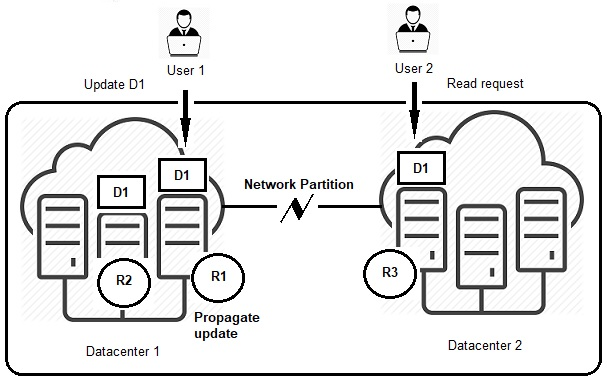
\includegraphics[width=0.47\textwidth]{fig1.jpg}
\caption{Consistency versus Availability in Replicated Systems.}
\label{fig:figure1}
\end{figure}

\vspace{1mm}
The realization of the trade-offs caused by the CAP theorem led to the proliferation of not-ACID models for building cloud-based applications, {\al {\it i.e.,}} systems that are {\al {\it Basically Available}}, rely on the maintenance of a {\al {\it Soft state} that can} be rebuilt in case of failures and are only {\al {\it Eventually consistent}} to be able to survive network partitions. %That 
{\al Such a} model became know as BASE~\cite{sosp1997base} and may offer different consistency models, which are discussed next. 
%in Section~\ref{sec:consistencymodels}.
\\
%\vspace{1mm}





\section{Consistency models}
\label{sec:consistencymodels}
%In this section, \textbf{we address the consistency models usually adopted by} distributed storage systems.
%we present the concepts of the consistency models in distributed storage systems.
%\textbf{First, we highlight the consistency perspectives} in this environment, and then we provide a hierarchical overview of the main consistency models.

%\subsection{Perspectives on Consistency}
%\subsection{Consistency Perspectives}

{\al A consistency model may be defined as a contract between a data storage system and the data processes that access it~\cite{tanenbaum:2007}. It defines strategies for supporting consistency within a distributed data storage system. However, trade-offs due to the CAP theorem require the choice from a range of models to address different consistency levels}, which may vary from a relaxed model to a strict one~\cite{bermbach2013consistency}. {\al In this context, there are two distinct perspectives to be considered in a distributed data storage system with respect to consistency}~\cite{tanenbaum:2007}: the \textit{data provider} and the {\al \textit{clients}}.
%In this context, there are two perspectives \textbf{in terms of consistency} to be considered in a distributed storage system \cite{tanenbaum:2007}: the \textit{provider} and the \textit{client}.
%demanding of the systems the need to incorporate a range of models that address consistency guarantees that varying from a relaxed consistency model to a strict consistency model \cite{bermbach2013consistency}. In this context, there are two perspectives to be considered on consistency in a distributed storage system \cite{tanenbaum:2007}: the provider and the client.

From the perspective of the data provider, the operations from all processes that want to access the data must be synchronized and ordered to guarantee correct results. From the perspective of the clients, it is often the case that shared updates are rare and they mostly access their private data. In that case, their major concern is that their own operations are consistent, what may be simpler to achieve.
%
%{\al The provider is responsible for synchronizing the processes {\dg that want to access} the replicas and ordering their operations.}
%%the synchronization processes among the replicas and the ordering of the operations. 
%The other perspective refers to the process of interaction between the client and the storage system. 
These two {\al consistency perspectives} are called \textit{data-centric} and \textit{client-centric}~\cite{tanenbaum:2007}. Next, we discuss the consistency models related to each {\al perspective}.
\vspace{2mm}

\subsection{Data-centric Consistency Models}
In this perspective, the consistency models seek to ensure that the data access process follows certain rules so that the storage system can work correctly. These rules are based on the definition of the results that are expected after read and write operations, even considering that these operations are concurrently performed. However, the absence of a global clock makes {\al the identification} of the last write operation a difficult task, %so that alternatively, it is required to apply 
which requires some restrictions on the data values that can be returned by a read operation, thus leading to a range of consistency models~\cite{tanenbaum:2007}.

The {\al consistency models that fall in this category %related to this perspective 
are:} \textit{weak consistency, PRAM consistency, causal consistency, sequential consistency and strict consistency}. 
%{\dg which are discussed next.} %{\rc  We describe each one of these models next}.
\vspace{1mm}

\subsubsection{Weak Consistency}

The weak consistency model offers the lowest possible ordering guarantee. As this guarantee is very weak, 
%it makes sense to affirm 
we can say that
it does not really exist, since an implementation may or may not have a protocol to synchronize replicas. It provides consistency to a group of transactions instead of to individual reads and writes, which is done by {\dg the} stricter consistency models 
{\dg that follow next} (PRAM, causal and sequential)~\cite{tanenbaum:2007, Vogels:2009}. % described next.
\vspace{1mm}

\subsubsection{PRAM Consistency}
 
PRAM (Pipelined Random Access Memory) consistency, also known as FIFO consistency, is a model in which write operations from a single process are seen by other processes in the same order that they were issued by its original process, whereas writes from different processes may be seen in a different order {\al by} different processes. In other words, there is no guarantee on the order in which the writes are seen by different processes, although writes from a single source must %arrive in order,
keep their order as if they were in a pipeline~\cite{lipton1988pram, tanenbaum:2007}.
\vspace{1mm}

\subsubsection{Causal Consistency}

Causal consistency is a model in which a sequential ordering is always maintained only between requests that have a causal relationship. Thus, concurrent requests do not share this relationship. In this case, all requests must be serialized in the same order on all replicas \cite{tanenbaum:2007}. {\al Thus, in a scenario of an always-available storage system in which requests have causal dependencies, a consistency level stricter than that provided by the casual model} cannot be achieved due to trade-offs of the CAP theorem~\cite{mahajan2011consistency}.

{\al More specifically,} two requests have a causal dependency if at least one of the following two conditions is achieved: (1) both requests are executed on a single thread and the execution of one precedes the other in time; (2) if a request B reads a value that has been written by a request A. Moreover, the relationship is transitive, so if A and B have a causal relation, and B and C also have a causal relation, then A and C share the same relationship~\cite{tanenbaum:2007, Vogels:2009}.
\vspace{1mm}

\subsubsection{Sequential Consistency}

Sequential consistency is a stricter  model that differs from the previous one in the sense that it extends to all requests %in order that 
the need of the replicas to agree on the ordering of non-causally related requests. It requires  that all operations be serialized in the same order on all replicas and that those related to the same process are executed in the order that they are received by the storage system~\cite{tanenbaum:2007}
%{\rc This model requires that the same serialization order imposed by the requests (verificar esta desri\c{c}\~ao)} is maintained on all replicas and the storage system must execute the requests in the order that they are received if they were sent by the same client~\cite{tanenbaum:2007}.
%\vspace{2mm}

\subsubsection{Strict Consistency}

Strict consistency is the model that provides the strongest consistency level. It states that if a write operation is performed on a data item, the result needs to be instantaneously visible to all processes, regardless in which replica the operation has occurred. To achieve this, an absolute global time order must be maintained~\cite{tanenbaum:2007}.
\\
%\vspace{3mm}

\subsection{Client-centric Consistency Models}

In this perspective, the distributed data store is characterized by an relative absence of simultaneous updates.
Also, when a simultaneous update occurs, the solution of any concurrency problem is simple to achieve.
%{\al Thus, in case that updates occur, there is no need to resolve them.}
%there are no problems in resolve them. 
The emphasis is then to maintain a consistent view of data items for an individual client process that is currently operating on the data store~\cite{tanenbaum:2007}. 
The models in this category are: \textit{eventual consistency, monotonic reads consistency, monotonic writes consistency, read-your-writes consistency} and \textit{writes-follow-reads consistency}. %{\rc We describe each one of these consistency models next.}
%\vspace{1mm}

\subsubsection{Eventual Consistency}

The eventual consistency model states that all updates will propagate through the system and all replicas will gradually become consistent in the case of the absence of updates for a long time \cite{tanenbaum:2007, Vogels:2009}. Although this model does not provide concrete consistency guarantees, there are several distributed storage systems that implement it~\cite{Chang06bigtable:a, decandia2007dynamo, Ghemawat2003Google, lakshman2010cassandra}.
\vspace{1mm}

\subsubsection{Monotonic Read Consistency}

The monotonic read consistency model guarantees that if a process reads a version of a data item \textit{d} at time \textit{t}, it will never see an older version of \textit{d} at a later time. In an scenario where data visibility is not guaranteed to be instantaneous, at least the versions of a data item will become visible in chronological order \cite{tanenbaum:2007, Vogels:2009}.
\vspace{1mm}

\subsubsection{Monotonic Write Consistency}

The monotonic write consistency model guarantees that a data store must serialize two writes \textit{$w_{1}$} and \textit{$w_{2}$} in the same order that they were sent by the same client~\cite{tanenbaum:2007, Vogels:2009}. For instance, if the initial write operation \textit{$w_{1}$} is lost, it is not allowed to the subsequent write \textit{$w_{2}$} to overwrite that data item.
\vspace{1mm}

\subsubsection{Read-Your-Writes Consistency}

Read-your-writes consistency is closely related to the monotonic reads model. It guarantees that once a write operation is performed on a data item \textit{d}, its effect will be seen by any successive read operation performed on \textit{d} by the same process~\cite{tanenbaum:2007, Vogels:2009}. This means that if a client has written a version \textit{v} of a data item \textit{d}, it will always be able to read a version at least as new as \textit{v}. 
%or upper.
\vspace{1mm}

\subsubsection{Writes-Follow-Reads Consistency}

Writes-follow-reads consistency guarantees that if a write operation \textit{w} is requested by a process on a data item \textit{d}, but there has been a previous read operation on \textit{d} by the same process, then it is guaranteed that \textit{w} will only be executed on the same or on a more recent value of \textit{d} previously read~\cite{tanenbaum:2007}.
\vspace{3mm}


\subsection{Hierarchical View of the Consistency \\ Models}
%https://www.overleaf.com/8967554ryqqdyzyrdcp#
In order to achieve a better understanding of the relationships among the consistency models, they can be hierarchically organized according to their degree of strictness from a lower consistency level to a higher one (see Figure~\ref{fig:hierarchicalView}).  

\begin{figure}[h]
\centering	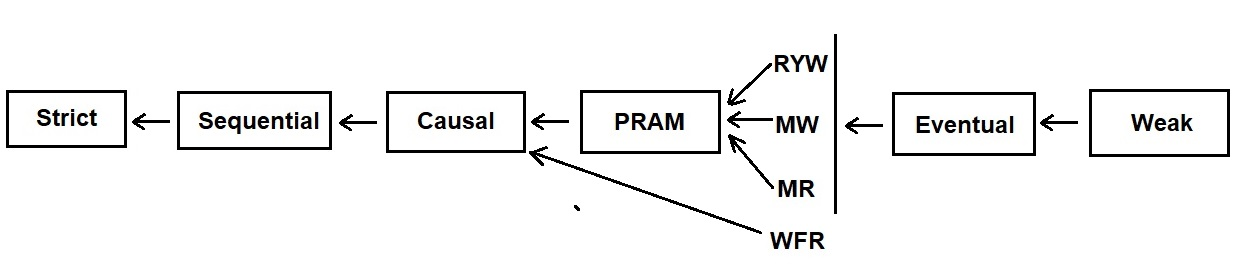
\includegraphics[width=0.48\textwidth]{fig2b.jpg}

\vspace{-3mm}
\caption{Hierarchical View of the Consistency Models.}
\label{fig:hierarchicalView}
\end{figure}
%\vspace{-1mm}

This hierarchical organization also considers some model combinations, such as the PRAM consistency model that may be seen as a combination of the monotonic read (MR), monotonic write (MW) and read-your-writes (RYW) models~\cite{bailis2013highly}. In addition, according to Brzezi\'nski et al.~\cite{brzezinski2004session}, there is also a relationship between causal consistency, which is a data-centric model, and the client-centric perspective,  
%and apparently, 
thus meaning that causal consistency is similar to write-follows-reads (WFR). 
%\vspace{2mm}
\\

\begin{comment}

\begin{figure}[h]
\centering
\begin{minipage}{18cm}
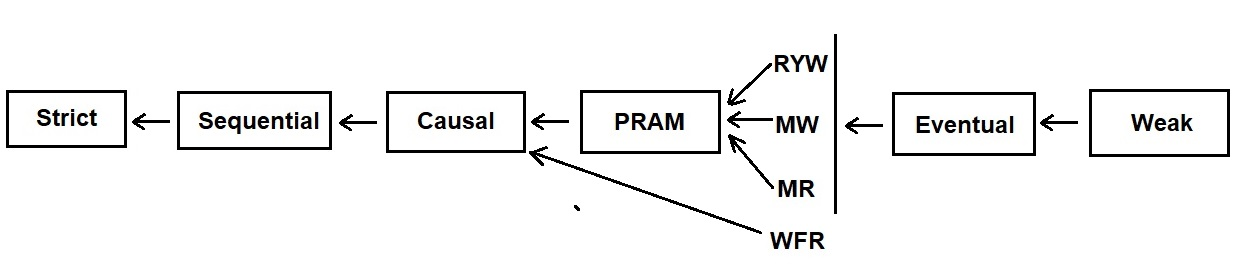
\includegraphics[width=0.43\textwidth]{fig2b.jpg}
\label{fig:fig2b}
\end{minipage}
\caption{Hierarchy of the Consistency Models}
\end{figure}
\end{comment}

\section{A Taxonomy for Consistency Methods}
\label{sec:taxonomy}
In this section, we propose a taxonomy for categorizing the various consistency methods addressed in this survey. The proposed taxonomy categorizes these methods as follows: \emph{static consistency methods, dynamic consistency methods, and consistency monitoring methods}. 

Our criteria for proposing this taxonomy are based on the similarities of the core ideas behind the methods, %in which we observed the common aspects in their approaches, 
which led us to consider these three categories as the most representative to categorize them. In what follows, we describe the main characteristics of the methods that belong to each category. 
\vspace{3mm}

\subsection{Static Consistency Methods}

This category includes those methods that provide consistency guarantees in cloud storage systems, but are not flexible enough to support self-adaptivity according to the applications' consisten\-cy requirements, \textit{i.e.}, such methods do not offer a diversity of consistency model options. Representative methods in this category are of two types: \textit{Event Sequencing-based Consistency} and \textit{Clock-bas\-ed Strict Consistency}, which have been  imple\-mented  in systems like PNUTS~\cite{cooper2008pnuts}, and  Spanner~\cite{Corbett:2013} and Clock-SI~\cite{Du2013}, respectively.
\vspace{3mm}

\begin{comment}

%This category includes those methods that rely on mechanisms proposed to provide consistency in cloud storage systems that {\al support service-oriented replication or partitioned data storage}. 
This category includes those consistency methods that rely on mechanisms that support service-oriented replication or partitioned data storage.
The predominant characteristic of these methods is that 
%the consistency guarantees 
they are not flexibile enough to support the clients' consistency requirements and, therefore, do not provide a diversity of consistency options. %in accordance to the Service Level Agreement (SLA).  
Representative methods in this category 
%{\rc are \textit{Event Sequencing-based Consistency} (PNUTS~\cite{cooper2008pnuts}) and \textit{Clock-bas\-ed Strict Consistency} (Spanner~\cite{Corbett:2013}, Clock-SI~\cite{Du2013})}.
{\al are of two types: \textit{Event Sequencing-based Consistency} and \textit{Clock-bas\-ed Strict Consistency}, which have been  imple\-mented  in systems like PNUTS~\cite{cooper2008pnuts}, and  Spanner~\cite{Corbett:2013} and Clock-SI~\cite{Du2013},  respectively}.

\end{comment}

\subsection{Dynamic Consistency Methods}

The methods in this category implement mechanisms that provide dynamic characteristics such as self-adaptive 
%consistency methods that automatically adjust the degrees of consistency 
or flexible consistency guarantees, which allows the selection or specification of the desired consistency level. 
%The methods included in this category 
They are of two types: \textit{Automated and Self-Adaptive Consistency,} and \textit{Flexible Consistency}. The first type has been implemented in systems like Harmony~\cite{chihoub2012harmony}, VFC$^3$~\cite{esteves2012quality} and Pileus \cite{Terry:2013}, whereas the second one supports systems like 
Indigo~\cite{balegas2015putting}, SSOR~\cite{Chen:2014} and Amazon DynamoDB~\cite{sivasubramanian2012amazon}. 
\vspace{3mm}

\subsection{Consistency Monitoring Methods}

Alternatively, instead of directly handling data consistency issues, some methods focus on providing mechanisms that allow data owners to detect the occurrence of consistency violations in the cloud storage. This means that 
%by {\al  using these} methods a group of clients might perform auditing on their data and make decisions based on how the Cloud Service Provider (CSP) stores and manages {\rc all data copies {\al  according to the consistency level that has been agreed upon} in  the service level contract. 
clients might audit their own data and make decisions based on how the Cloud Service Provider (CSP) stores and manages their data copies according to the consistency level that has been agreed upon in  the service level contract. 
The methods in this category are of two types, \textit{Consistency Verification} and \textit{Consistency Auditing}, and have been respectively implemented in VICOS~\cite{BrandenburgerCK15}, and in DMR-PDP~\cite{MukundanML12} and CaaS~\cite{liu2014consistency}.
\vspace{3mm}


\section{Overview of Cloud Database Consistency Methods}
\label{sec:overview}
In this section, we present an overview of 
%the types of strategy 
the main approaches adopted %strategies provided 
by the consistency methods addressed in this survey. These methods are among the most representative in the literature, although our survey is not exhaustive. The presentation follows the taxonomy introduced in Section~4. 
%In this section, {\al we present an overview of the consistency methods we address in this survey. {\rc The approach of each method is based on the description of the systems we have found in the literature that implement them.} These methods are among the most representative in the literature, although our survey is not exhaustive. The presentation below follows the taxonomy introduced in Section~4.}
\vspace{1mm}

\subsection{Static Consistency Methods}

As mentioned earlier, the methods in this category provide fixed guarantees, not being able, for example, to adjust their behavior to take advantage of situations where a stronger consistency might be temporarily available. {\al As we shall see next,} {\dg they can be divided into two types: those based on the sequence of events and those based on clock timestamps.} %{\rc We discuss them next.}
\vspace{1mm}

\subsubsection{Event Sequencing-based Consistency}

This type of consistency method aims to hide the replication complexity by providing a consistency model that lies between the two extremes of general serializability and eventual consistency. The key aspect behind this type of method is the observation that 
%serializability os transactions is inefficient
transaction serializability is costly and often unnecessary in web applications~\cite{cooper2008pnuts}.

The most representative system that implements this type of method is PNUTS~\cite{cooper2008pnuts}, which is a massively parallel and geographically distributed DBMS developed by Yahoo for web applications. PNUTS developers observed that web applications typically manipulate one record at a time, whereas different records may be located in different geographic locality. Hence, an event sequencing-based consistency method establishes that all replicas of a given record receive all updates applied to that record in the same order. This strategy is implemented by designating one of the replicas as the master for each record, so that this master receives all writes sent to that record by the other replicas. If a record has the majority of its writes sent to a particular replica, this replica becomes the master for that record.
\vspace{1mm}

%PNUTS \cite{cooper2008pnuts} is a massively parallel and geographically distributed DBMS  developed for Yahoo!’s web applications. It provides several features such as scalability, high availability and fault tolerance, and relaxed consistency guarantees. Although many distributed replicated data storage systems choose to provide eventual consistency, PNUTS offers an {\rc event sequencing-based consistency method}, {\al since the eventual consistency model is often too weak and unappropriated for web applications \cite{cooper2008pnuts}.This consistency method aims to hide the replication complexity, thus providing a consistency model that is between the two extremes of general serializability and eventual consistency.} 

%The key aspect of this method is the observation that serializability of general transactions is inefficient and often unnecessary in web applications. On the other hand, enforcing only eventual consistency where all updates will eventually be applied {\al in a different order on different replicas} is also inadequate for web applications. The PNUTS' developers observed that {\al web applications typically manipulate one record at a time whereas different records may have activity with different geographic locality~\cite{cooper2008pnuts}.} Hence, their method establishes that all replicas of a given record apply all updates to the record in the same order. 

%The per-record timeline consistency method is implemented by 
%the establishment of one of the replicas to be designated 
%\al  designating one of the replicas as the master for each record so that this master receives all updates to that record that were sent by the other replicas.} If a record has the majority of its writes sent to a particular replica, this replica will become the master for that record.\\

\subsubsection{Clock-based Strict Consistency}

Systems that implement this type of consistency method are characterized by the use of clock-based mechanisms to control timestamps to enforce strict consistency \cite{Corbett:2013, Du2013}. They offer the guarantee that arbitrary objects in the data store are accessed atomically and isolated from concurrent accesses. 
%For that, it is provided strong semantics with general purpose transactions, supporting read and write operations.
The approach behind this consistency method is based on the  
ability of a system to provide a timestamp log to track the order in which operations occur. 
%In some distributed DBMS, a timestamp-based algorithm is used for controlling concurrency allowing to safely handle transactions.

Spanner \cite{Corbett:2013} and Clock-SI \cite{Du2013} are representative systems that implement this type of consistency method. The former is a relational-like distributed data store system developed by Google. It assigns globally-meaningful commit timestamps that reflect the serialization order of the transactions, which may be distributed. Spanner also enforces that if a transaction \textit{T$_{2}$} begins after the commit of a transaction \textit{T$_{1}$}, then the commit timestamp of \textit{T$_{2} $} must be greater than the commit timestamp of \textit{T$_{1}$}.

%{\color{green}It assigns commit timestamps that reflect the serialization order of the transactions. Hence, a commit operation receives a timestamp \emph{C} to update once a transaction acquire all the locks. In addition, a read-only operation receives a timestamp \emph{S} by reading the local physical clock. Operations assigned to a timestamp \emph{S} that are related to a same physical timestamp \emph{T} are blocked by Spanner in case it cannot yet be ensured that no new operations assigned to a timestamp \emph{C} will be able to perform with \textit{T'} <~\textit{T}. Obs: Na discussão acima, as variáveis $C, S, T, T'$ não ajudam na descrição do método pois não há nenhuma relação entre elas.}

On the other hand, Clock-SI implements the so called \textit{snapshot isolation}, which is a consistency criterion for partitioned data storages. In this strategy, read-only operations read from a consistent snapshot and other operations perform a commit if no objects written by these transactions were
concurrently written. The local physical clock is used by each transaction to identify its read timestamp.
\vspace{1mm}

%Clock-SI \cite{Du2013} and Spanner \cite{Corbett:2013} are {\al data store} systems that use clock-based mechanisms to control timestamps to enforce strict consistency. They offer the guarantee that arbitrary objects in the data store will be accessed atomically and isolated from concurrent accesses. For that, both solutions provide strong semantics with general purpose transactions, supporting read and write operations. The approach of using the system's clock is based on the system's ability to perform timestamp event log to track the order in which they occur. In some distributed DBMS, a timestamp-based algorithm is used for controlling concurrency allowing to safely handle transactions. 

%Clock-SI \cite{Du2013} implements the so called \textit{Snapshot Isolation} (SI), which is a consistency criterion for partitioned data storage. In this mechanism, read-only operations read from a consistent snapshot and other operations perform commit if no objects written by these transactions were also written concurrently. The local physical clock is used by each transaction in order to identify its read timestamp.

%Spanner \cite{Corbett:2013} is Google’s {\al relational-like distributed data store system} that supports scalable, globally-distributed and replicated databases. It assigns a timestamp \emph{S} to possibly read-only operations by reading the local physical clock. Equivalently, it assigns a commit timestamp \emph{C} to update operations once that these transactions acquire all the locks over the write-set \emph{W}, which is then used to version the new data items. Moreover, read transactions related to a physical timestamp \emph{T} are blocked by Spanner in case it cannot yet be ensured that no new update operation will be able to perform a commit with a timestamp \textit{T'} < \textit{T}.

\subsection{Dynamic Consistency Methods}

Some methods may be able to adjust guarantees based on the observation of access patterns and {\al system structural aspects. We discuss them next.}

\vspace{2mm}
\subsubsection{Automated and Self-adaptive Consistency}

This type of consistency method aims to dynamically enforce multiple consistency degrees over distinct data objects.  
Three main approaches %strategies %related to
have been adopted to implement such methods. 

%{\rc  probabilistic computation~\cite{chihoub2012harmony}, consistency vector \cite{esteves2012quality} and dynamic server selection}~\cite{Terry:2013}. 

The first approach is based on probabilistic computations that provide an estimation of the stale reads rate. Once the estimation model is computed, it is possible to identify the key parameter that affects the stale reads and scale up/down the number of replicas involved in read operations in order to maintain a low tolerable fraction of stale reads. This approach is mainly implemented by Harmony~\cite{chihoub2012harmony}, which is a consistency-based system that aims to gradual and dynamically tune the consistency level at runtime according to the applications' consistency requirements.

The second approach allows the evaluation and enforcement of divergence bounds over data objects (table/row/column), so that the consistency levels can be automatically adjusted based on statistical information. The evaluation takes place on a divergence vector every time an update request is received, although it is necessary to identify the affected data objects. If any limit is exceeded, all updates since the last replication are placed in a FIFO-like queue to be propagated and executed on other replicas. 
%allows the definition and dynamic enforcement of multiple consistency degrees over different groups of data, within the same application, across very large scale networks of cloud data centers. This model is driven by the different semantics that data might have, and the consistency levels can be automatically adjusted based on statistical information.
%of three-dimensional consistency vectors that can be associated with {\rc data objects.
%each data item. 
%These vectors ($\kappa$) are used to bound the maximum objects divergence, which is represented by a numerical scalar associated to the three orthogonal constraints: Time ($\theta$), Sequence ($\sigma$) and Value ($\nu$).}
%The constraint time ($\theta$) specifies the maximum time a replica can be without being updated with is latest value. {\rc Thus, given a data object \textit{o}, by the constraint $\theta$(\textit{o}) can be obtained the time (e.g., seconds) passed since the last replica update of this data object.}
%The constraint sequence ($\sigma$) specifies the maximum number of updates that can be applied to an object without refreshing its replicas. {\rc Thus, given a data object \textit{o}, by the constraint $\sigma$(\textit{o}) can be obtained the number of applied updates to this data object.} 
%Finally, the constraint value ($\nu$) specifies the maximum relative difference between replica contents or against a constant, {\rc capturing the impact or importance of updates on the data object’s internal state. Thus, given a data object \textit{o}, by the constraint $\nu$(\textit{o}) can be obtained that difference (e.g., in percentage).}  
%Once it is specified the intervals of values on the vectors ($\kappa$), the consistency intensity is automatically adjusted. {\rc  
%This adjustment is based on the observation of the frequency of read and write transactions.} 
The most representative system that implements 
%framework that implements 
this approach is VFC$^3$ (\textit{Versatile Framework for Consistency ~in Cloud Computing})~\cite{esteves2012quality}, which provides three-dimensional consistency Qual\-ity-of-Service vectors, where users can specify consistency parameters according to the QoS level desired, thus letting the system automatically adjust the consistency degree.
% a consistency model that aims to enforce increasing degrees of consistency for different types of data.

Finally, the third approach is characterized by dynamically selecting to which server (or even set of servers) each read of a record must be directed, so that the best service is delivered given the current configuration and system conditions. Hence, this approach is adaptable to distinct configurations of replicas and users, as well as to changing conditions such as variations on the network performance or server load. Another important aspect of this approach is the fact that it allows application developers to provide a Service Level Agreement (SLA) that specifies the applications' consistency/latency desires in a declarative manner. Pileus~\cite{Terry:2013} is a key-value storage system that implements this approach. It provides a diversity of consistency guarantee options for globally distributed and replicated data environments. It also allows several systems or even clients of a system to achieve different consistency degrees, even while sharing the same data.

\begin{comment}
Harmony \cite{chihoub2012harmony} is a consistency-based system that aims {\al to gradually and dynamically} tune the consistency level at runtime {\rc  according to the applications' consistency requirements.} It also %aims to
{\al handles specific} issues related to data consistency, such as network latency, that directly affect {\al the propagation of updates to replicas}, and the frequency of access patterns during reads, writes and updates, which represents the application’s demands. These issues may increase the probability of stale reads and Harmony {\al aims to specifically reduce this.}

The self-adaptive consistency method proposed by Harmony is based on probabilistic computations that provide an
estimation of the stale reads rate. Once the estimation model is computed, it is possible to identify the key parameter that is affecting the stale reads, and scale up/down the number of replicas involved in read operations in order to maintain a low tolerable fraction of stale reads.

Pileus~\cite{Terry:2013} is a key-value storage system that provides a diversity of consistency {\al guarantee options for globally distributed and replicated data environments.} %by a method of selection of consistency guarantees, which are located between a strict and eventual consistency level. It allows several systems or {\al even clients} of a system to achieve different consistency {\al guarantee levels}, even while sharing the same data. Pileus {\al aims to} reduce the responsibility of system developers of {\al having to explicitly choose} a single ideal con\-sist\-en\-cy level. This is a very significant feature due to the problem {\al  imposed by} multi-consistency storage services, in which {\al system developers} must decide at development time which consistency level to adopt. {\al Since different clients require distinct performance and consistency levels for their applications,} it is difficult to choose a consistency-performance pair that satisfies all clients in a wide range of scenario.

{\al Thus, to overcome this difficulty, Pileus allows application developers to provide a Service Level Agreement (SLA) that specifies the application’s consistency/latency desires in a declarative manner~\cite{Terry:2013}.} 
%The proposed method uses Service Level Agreements (SLA) in which is specified the system’s consistency/latency desired level in a declarative manner. 
An SLA may indicate a large range of acceptable consistency/latency trade-offs. Pileus dynamically selects to which server, or even a set of servers, each read is directed, so that the best service is delivered given the current configuration and system conditions. Hence, it adapts to distinct configurations of replicas and users, as well as to changing conditions, including variations in network or server load.

Versatile Framework for Consistency
in~~Cloud Computing (VFC$^3$) \cite{esteves2012quality} {\al is} a consistency model that aims to enforce increasing degrees of consistency for different types of data. 
%based on their semantics.
{\al It provides different} degrees of consistency that can be automatically adjusted based on statistical information, {\al being particularly suitable to large-scale and dynamic environments that need to syncronize large amounts of data over several geographically dispersed points.}
%in case of these environments have large amounts of data to be synchronized and there are several geographically dispersed points.

The key aspect of VFC's consistency method is the definition of three-dimensional consistency vectors ($\kappa$) that can be associated with data items. Time ($\theta$) specifies the maximum time a replica can be without being updated with is latest value. Sequence ($\sigma$) specifies the maximum number of updates that can be applied to an object without refreshing its replicas. Value ($\nu$) specifies the maximum relative difference between replica contents or against a constant, thus it captures the impact or importance of updates on the data items’ internal state. Once a client specify the intervals of values on the vectors ($\kappa$), VFC automatically adjust the consistency intensity. To perform this adjustment the VFC's Quality of Service (QoS) engine component observes the frequency of read and write operations to data items during a given time frame.
\end{comment}

\vspace{-0.2mm}
\subsubsection{Flexible Consistency}

This type of consistency method is characterized by its flexibility to adapt to predefined consistency models. In this context, there are three main approaches that implement this type of consistency: combining %the} %strengths of 
both weak and strong consistency depending on the operation, adopting the notion of consistency regions and performing eventually or strongly consistent reads as needed~\cite{balegas2015putting, Chen:2014, sivasubramanian2012amazon}.

The first approach aims to strengthen eventual consistency allowing the applications to specify consistency rules, or \textit{invariants}, that must be maintained by the system. Once these invariants are defined, it is possible to identify the operations that are potentially unsafe under concurrent execution, thus allowing one to select either a violation-avoid\-ance or an invariant-repair technique. Indigo \cite{balegas2015putting} is a middleware system that implements this approach. %strategy. 
%It was designed to implement 
It supports an alternative consistency method %that was 
built on top of a geo-replicated key-value data store.

The second approach is based on a formalism proposed to support the applications’ consistency requirements. The trade-off between consistency and scalability requirements is handled by introducing the notion of consistency regions and service-delivery-oriented consistency policies. A consistency region is defined as a logical unit that represents the application state-level requirements for consistency and scalability. This concept is used to define consistency boundaries that separate each group of services that need to be ordered. Hence, services that need to be kept consistent must be associated to a certain region. The definition of what region a service belongs to and which services that can concurrently be delivered is set by the system administrators. 

\textit{Scalable Service Oriented Replication} (SSOR) \cite{Chen:2014} is a middleware that implements this approach. %strategy. 
It covers three distinct types of consistency region: (1)~Conflict Region (CR), which is a region composed by services that have conflicting requirements for consistency regardless of the session; (2) Sessional Conflict Region (SCR), which is a region that includes services of a particular session with conflicting consistency requirements; and (3) Non-Con\-flict Region (NCR), which is a region that does not impose any consistency constraints or requirements.

The third approach aims to provide elasticity and flexibility in order to handle unpredictable workloads, but allowing a system to be tuned for capacity. Due to this characteristic, it allows applications to perform eventually or strongly consistent reads as needed. Amazon DynamoDB~\cite{sivasubramanian2012amazon} is a highly reliable and cost-effective NoSQL database service that implements this  approach. %consistency strategy. 
It was built based on the experience with its predecessor Dynamo~\cite{decandia2007dynamo}. DynamoDB adopts %the eventual consistency option
eventual consistency as its default model, which does not guarantee that an eventually consistent read will always reflect the result of a recently completed write. On the other hand, when adopting a stronger consistency model, it returns a result that reflects all writes that have received a successful response prior to that read. \\
%\vspace{4mm}

\begin{comment}
The Scalable Service Oriented Replication (SSOR) solution \cite{Chen:2014} is a middleware based on a formalism proposed to address the applications’ consistency requirements and flexibly adapt to predefined consistency models. The trade-off between consistency and scalability requirements is handled by the introducing of the notion of consistency regions and service delivery oriented to consistency policies.

A consistency region is defined as a logical unit to represent the application state-level requirements for consistency and scalability. A component or application that consists of a number of services (service group) may consist of many regions, and each region contains one or more services. This concept is used to define consistency boundaries that separate each group of services that need to be ordered. Hence, services that need to be kept consistent must be associated to a certain region. The definition of what region a service belongs to and which services can concurrently be delivered is set by the systems administrators. Posteriorly, the consistency policies can then be used to coordinate corresponding reactions at the communication level protocols among the replicas.

SSOR covers three distinct types of consistency region: (1) Conflict Region (CR) is a region composed by services that have conflicting requirements for consistency regardless of the session; (2) Sessional Conflict Region (SCR) is a region that includes services of a particular session with conflicting consistency requirements; Non-conflict Region (NR) is a region that does not impose any consistency constraints or requirements.

Amazon DynamoDB \cite{sivasubramanian2012amazon} is a highly reliable and cost-effective NoSQL database service that {\al was} built based on the experience with its predecessor Dynamo~\cite{decandia2007dynamo}. Among other features, it was designed to provide high scalability for {\al large} Internet applications, {\al thus providing both} elasticity and flexibility in order to handle unpredictable workloads, {\al but allowing a system to tune for capacity.} Due {\al to this characteristic, it allows} applications to perform eventually or strongly consistent reads as needed.

{\color{green}
\noindent
\textbf{(Versão anterior)}\par
DynamoDB adopts an eventual consistency as default model and maximizes the read throughput, although it is not guaranteed that an eventually consistent read will always reflect the results of a recently completed write. On the other hand, if a strongly consistent read is chosen, it is returned a result that reflects all writes that received a successful response prior to the read. To get this result it is possible to specify optional parameters in a request, which imply that a strongly consistent read will take more resources to be processed than an eventually consistent read.

Indigo \cite{balegas2015putting} is a middleware system designed to implement an alternative consistency method, so called \textit{Explicit Consistency} that has built on top of a geo-replicated key-value data store. This model aims to strengthen eventual consistency allowing the applications to specify consistency rules, or \textit{invariants}, that must be assuredly maintained by the system. Once these invariants that should be met are defined, the consistency method implemented by Indigo identifies the operations that are potentially unsafe under concurrent execution, and then one can select either violation-avoidance or invariant-repair techniques.

The Indigo's approach is based on the supporting both weak and strong consistency, depending on the operation. Strong application invariants are guaranteed when it is needed, whereas it provides similar latency to an eventually-consistent system in the remain cases. Instead of to define consistency in terms of execution orders, the Indigo's consistency method define it in terms of application properties. Provided that the specified invariants are not affected, the system is free to reorder execution of operations at different replicas.
}

{\rc  
\noindent
\textbf{(versão atual)}\par
DynamoDB adopts the eventual consistency option as its default model, where it is not guaranteed that an eventually consistent read will always reflect the results of a recently completed write. On the other hand, in a strongly consistent read option, it is returned a result that reflects all writes that received a successful response prior to the read.

Indigo \cite{balegas2015putting} is a middleware system designed to implement an alternative consistency method, called \textit{Explicit Consistency}, that was built on top of a geo-replicated key-value data store. The approach behind this method is based on the attempt to combine the strengths of both weak and strong consistency, depending on the operation.

Indigo aims to strengthen eventual consistency allowing the applications to specify consistency rules, or \textit{invariants}, that must be maintained by the system. Once these invariants are defined, the consistency method implemented by Indigo identifies the operations that are potentially unsafe under concurrent execution, thus allowing one to select either a violation-avoidance or a invariant-repair technique. Instead of defining consistency in terms of execution orders, Indigo defines it as application properties. Thus, provided that the specified invariants are not affected, the system is free to reorder the execution of operations at different replicas.
}
\end{comment}

\vspace{-1mm}
\subsection{Consistency Monitoring Methods}

The methods in this category  
%provide means for 
allow the applications to evaluate the level of consistency that has been actually obtained during execution, so that they can make their own decisions on how to handle any problems when they arise. 
% Acho que aqui não precisa dessa frase, pois o parágrafo já começa com "the methods in this cathegory", o que funciona como uma introdução para o que vem depois.
% {\al We discuss them next.}

\subsubsection{Consistency Verification}

These methods rely on two approaches to consistency verification. The first consists of a protocol that enables a group of mutually trusting clients to detect consistency violations on a cloud storage, whereas the second provides a verification scheme that allows data owners to ensure whether the Cloud Service Provider (CSP) complies with the SLA for storing data in multiple replicas.

%The protocol is implemented by VICOS
This protocol-based approach is adopted by VICOS (Verification of Integrity and Consistency for Cloud Object Storage)~\cite{BrandenburgerCK15}. VICOS supports the optimal con\-sist\-ency concept of \textit{fork-linearizability}, which captures the strongest achievable notion of consistency in multi-client models. The method may guarantee this notion by registering the causal evolution of the user’s views into their interaction with the server. In case the server creates only a single discrepancy between the views of two clients, it is ensured that these clients will never observe operations of each other afterwards. That is, if these users communicate later and the server ever lies to them, the violation will be immediately discovered. Thus, users can verify a large number of past transactions by performing a single check.

The verification approach is implemented by DMR-PDP~(\textit{Dynamic Multi-Replica-Pro\-vable Data Possession}) \cite{MukundanML12}. The context addressed by this scheme is that whenever data owners ask the CSP to replicate data at different servers, they are charged for this. Hence, data owners need to be strongly persuaded that the CSP stores all data copies that are agreed upon in the service level contract, as well as that all remotely stored copies correctly execute the updates requested by the users. %The proposed 
This approach deals with such problems by preventing the CSP from cheating the data storage; for instance, by maintaining fewer copies than paid for. The scheme is based on a technique called \textit{Provable Data Possession}~\cite{ateniese2007provable}, used to audit and validate the integrity and consistency of data stored on remote servers.

%Verification of Integrity and Consistency for Cloud Object Storage (VICOS) \cite{BrandenburgerCK15} is a protocol that enables a group of mutually trusting clients to detect data-integrity and consistency violations for cloud storage. It extends the standard idea of linearizability in distributed systems. In shared and distributed memory, this criterion is usually called atomic consistency and requires that the execution of a set of operations by all clients together is equivalent to a sequential execution, respecting the real-time ordering of the operations. 

%VICOS supports the optimal consistency concept of \textit{fork-linearizability}, which captures the strongest achievable notion of consistency in multi-client models. The method may guarantee this notion by registering the causal evolution of the user’s views into their interaction with the server. In case the server creates only a single discrepancy between the views of two clients, it is ensured that these clients will never observe operations of each other afterwards. That is, if these users communicate later and the server ever lies to them, the violation will be immediately discovered. Thus, the users can verify a large number of past transactions by performing a single check.

%Dynamic Multi-Replica Provable Data Possession (DMR-PDP) \cite{MukundanML12} is a scheme that allows data owners to ensure whether the Cloud Service Provider (CSP) complies with the service level agreement for storing data in multiple replicas. 

%Whenever data owners ask the CSP to replicate data at different servers, they are charged for this. Hence, data owners need to be strongly persuaded that the CSP stores all data copies that are agreed upon in the service level contract, as well as that all remotely stored copies correctly execute the updates requested by the users. The proposed method aims to deal with such problems by preventing the CSP from cheating the data storage; for instance, by maintaining fewer copies than it was paid for. The scheme is based on a technique called \textit{Provable Data Possession} (PDP)~\cite{ateniese2007provable}, which is used to audit and validate the integrity and consistency of data stored on remote servers.

\vspace{1mm} 
\subsubsection{Consistency Auditing}

This {\al kind of method is based on an architecture that %comprehends} 
conists of} a large data cloud maintained by a {\al CSP}
%Cloud Service Provider (CSP) 
and multiple small audit clouds composed of a group of users that cooperate on a specific job ({\it e.g.}, {\al revising} a document or {\al writing} a program). The required level of consistency that should be provided by the data cloud is stipulated by {\al an SLA} 
%Service Level Agreement (SLA) 
involving the audit cloud and the data cloud. Once the SLA exists, the audit cloud can verify whether the data cloud violates {\al it}, thus quantifying, in monetary terms or otherwise, the severity of the violation.

Consistency as a Service (CaaS) \cite{liu2014consistency} implements this method. It relies on a two-level auditing structure, name\-ly: \textit{local auditing} and \textit{global auditing}. Local auditing allows each user to independently perform local tracing operations, focusing on monotonic read and read-your-write consistencies. Global auditing, on the other hand, requires that an auditor is periodically elected from the audit cloud to perform global tracing operations, focusing on casual consistency. This type of method is supported by constructing a directed graph of operations, called the \textit{precedence graph}. If the constructed graph is a directed acyclic graph (DAG), the required level of consistency is preserved~\cite{liu2014consistency}.


%Consistency as a Service (CaaS) \cite{liu2014consistency} is a model that consists of a large data cloud maintained by a Cloud Service Provider (CSP) and multiple small audit clouds composed of a group of users that cooperate on a specific job (e.g., a document or a program). The required level of consistency that should be provided by the data cloud is stipulated by a Service Level Agreement (SLA) involving the audit cloud and the data cloud. Once the SLA exists, the audit cloud can verify whether the data cloud violates the SLA, thus quantifying, in monetary terms or otherwise, the severity of the violations.

%CaaS relies on a two-level auditing structure, name\-ly: \textit{local auditing} and \textit{global auditing}. Local auditing allows each user to independently perform local tracing operations, focusing on monotonic read and read-your-write consistencies. Global auditing, on the other hand, requires that an auditor is preodically elected from the audit cloud to perform global tracing operations, focusing on casual consistency. This type of consistency is supported by constructing a directed graph of operations, called the \textit{precedence graph}. If the constructed graph is a directed acyclic graph (DAG), the required level of consistency is preserved~\cite{liu2014consistency}.


\section{Discussion}
\label{sec:discussion}
\begin{table*}[t]
	\centering
	\setlength\tabcolsep{4pt}
	\caption{Storage Requirements Supported by the Consistency Methods}
	\label{tab:storageRequirements}
	\begin{tabular}{|c|c|l|l|l|l|l|l|l|l|}
		\hline
		Category & Representative Systems  & \multicolumn{8}{|c|}{Storage Requirements
        {\al {\cite{ju2011survey, rimal2009taxonomy}}}} \\
		\hline
		&                 & 
		\rotatebox{90}{Automation} &  
		\rotatebox{90}{Availability} & 
		\rotatebox{90}{Elasticity} & 
		\rotatebox{90}{Fault Tolerance~} & 
		\rotatebox{90}{Low-Latency}  & 
		\rotatebox{90}{Performance} &  
		\rotatebox{90}{Reliability} & 
		\rotatebox{90}{Scalability}\\ 
		\hline   
		
		\multirow{3}{*}{ \begin{tabular}[c]{@{}c@{}} Static Consistency \\ Methods \end{tabular}}                & 
		PNUTS \cite{cooper2008pnuts}     &  & \checkmark &   & \checkmark &  &   & \checkmark & \checkmark  \\ \cline{2-10} 
		& Spanner \cite{Corbett:2013} &  & \checkmark &  & \checkmark  & \checkmark &  &  & \checkmark \\ \cline{2-10}
		& Clock-SI \cite{Du2013} &  & \checkmark &  &  & \checkmark & \checkmark &  & \checkmark \\
		\hline \hline
		
		\multirow{6}{*}{ \begin{tabular}[c]{@{}c@{}} Dynamic Consistency \\ Methods \end{tabular}}    & 
		Indigo \cite{balegas2015putting} &  &  &  & \checkmark & \checkmark &  &  &   \\ \cline{2-10} 
		& SSOR \cite{Chen:2014} &  &  & \checkmark & \checkmark &   & \checkmark  & \checkmark & \checkmark  \\ \cline{2-10} 
		& Harmony \cite{chihoub2012harmony} & \checkmark & \checkmark  & \checkmark &  & \checkmark & \checkmark  &   &  \\ \cline{2-10}
		& VFC \cite{esteves2012quality} & \checkmark & \checkmark  &   &  & \checkmark & \checkmark & \checkmark & \checkmark  \\ \cline{2-10}
		& DynamoDB \cite{sivasubramanian2012amazon} &   & \checkmark & \checkmark  &   & \checkmark & \checkmark & \checkmark & \checkmark  \\ \cline{2-10}
		& Pileus \cite{Terry:2013} & \checkmark & \checkmark &   & \checkmark &  & \checkmark & \checkmark & \checkmark  \\ \hline \hline
		
		\multirow{3}{*}{ \begin{tabular}[c]{@{}c@{}} Consistency Monitoring \\ Methods \end{tabular}}    & 
		VICOS \cite{BrandenburgerCK15} &  \multicolumn{8}{|c|}{not applied}   \\ \cline{2-10} 
		& CaaS \cite{liu2014consistency} &  \multicolumn{8}{|c|}{not applied}  \\ \cline{2-10} 
		& DMR-PDP \cite{MukundanML12} &  \multicolumn{8}{|c|}{not applied}  
		\\ \hline 
	\end{tabular}
\end{table*}

\begin{comment}
{\color{yellow}
\noindent
\textbf{(versão anterior)}\par
In the category of consistency guarantee methods, we have described the \textit{per-record timeline consistency} method \cite{cooper2008pnuts}. This method was designed in order to achieve the Yahoo!’s applications consistency requirements, thus it is based on the experience with many web applications. The main contribution of this method is the conception that in a scenario of replicated data storage in web applications, consistency can be achievable by the control of events (inserts, updates and deletes) in a timeline. This control is based on a sequence number that consists of the generation and the versioning of the record, where each update of an existing record implies a new version. A consistent version from the timeline is returned if a read operation is performed of any replica, which always move forward in the timeline.

The approach of object versioning is also exploited by the clock-based strict consistency method. Clock-SI \cite{Du2013} and Spanner \cite{Corbett:2013} capture similar idea in the ordering of events by the exploitation of clock-based mechanisms in order to keep track of the ordering of transactions.

We observe that the ordering of events is a well-understood approach in distributed systems \cite{fidge1991logical, lamport1978time, mattern1989virtual}. The concept of one event happening before another represents a causal relationship and the total ordering of this events can be used for solving synchronization issues, so that the methods above described extend this concept on their particular approaches.

In the category of consistency auditing methods we have described \textit{consistency verifying protocols}  \cite{BrandenburgerCK15, MukundanML12}   and \textit{consistency auditing}\cite{liu2014consistency}. In general, these methods are suitable for scenarios where multiple clients cooperate on a remotely data stored in a potentially misbehaving service, and they need rely on the cloud service provider regarding the confidentiality and correctness of their data. Furthermore, these clients need to verify if the data updates that are requested are correctly executed on all remotely stored copies, whereas the consistency level required is maintained.

Regarding the dynamic consistency methods there are \textit{automated and self-adaptive consistency} \cite{chihoub2012harmony, esteves2012quality, Terry:2013} and \textit{flexible consistency guarantees} methods \cite{Chen:2014, sivasubramanian2012amazon}. Instead of to apply the same consistency guarantee methods' approach, the automated and self-adaptive are focused in achieve automaticity in their consistency guarantees by the use of mechanisms that adjust the degrees of consistency without human intervention. This is an important feature for applications that have temporal characteristics, which require dynamic adjustment in the consistency requisites of data over time and real-time workload cloud storage systems. Moreover, the flexible guarantees approach seeks to address the applications’ consistency requirements and flexibly adapt to predefined consistency models.
}
\end{comment}

\vspace{2mm}
As proposed in Section~4, consistency methods can be grouped in three categories: static consistency methods, dynamic consistency methods and consistency monitoring methods.

Static Consistency methods are mostly based on versioning of events. This captures the idea of event ordering by means of control strategies such as a sequence number that represents a data object version or clock-based mechanisms. We note that this is a well-understood concept in distributed systems~\cite{fidge1991logical, lamport1978time, mattern1989virtual}. The idea of an event happening before another represents a causal relationship and the total ordering of events among the replicas has been shown quite useful for solving synchronization issues related to data consistency. Thus, consistency methods in this category extend this concept on specific scenarios.

Dynamic consistency methods, in turn, generally aim to provide mechanisms that adjust the degree of consistency without human intervention. This is an important feature for applications that have temporal characteristics, 
%which requires the dynamic adjustment of the consistency requirements overtime, 
as well as for real-time workload cloud storage systems. Specifically, flexible consistency methods are suitable to address applications’ consistency requirements that need to adapt to predefined consistency models.

On the other hand, consistency monitoring methods do not provide specific guarantees, but focus on detecting the occurrence of consistency violations in the cloud data storage.  Despite that, these methods offer significant contributions that are suitable for scenarios where multiple clients cooperate on data remotely stored in a potentially misbehaving service, and need to rely on the Cloud Service Provider to guarantee their confidentiality and correctness. Furthermore, those clients need to verify if the requested data updates 
%that are 
{\al were} correctly executed on all remotely stored copies, while maintaining the required consistency level.

Finally, Table~\ref{tab:storageRequirements} summarizes the storage requirements supported by the systems that we have surveyed in order to stress what are the main consistency trade-offs considered by them. Note that we only address those systems that implement %consistency guarantee and dynamic consistency 
a specific consistency method, since consistency monitoring methods only focus on detecting consistency violations. 
%so that in the Table~1 the storage requirements are not applied to the consistency auditing category. 
Table~\ref{tab:storageRequirements} also shows that availability and scalability are the most addressed storage requirements supported by the surveyed system, whereas elasticity is the least one. 
%is not widely addressed by them.} 

As previously mentioned, existing trade-offs determined by the CAP theorem imply that applications must sacrifice consistency under certain scenarios to be able to satisfy other application requirements. This suggests that most of the consistency methods are also involved in providing other features such as high availability and scalability, even reducing the degree of consistency to a level that may be deemed acceptable.

Although elasticity is not exploited by most of the surveyed systems, this is a desirable and important feature for large scale applications. It is characterized by the ability to deal with load increases by adding more resources during high demand and releasing them when load decreases. {\rc Elasticity differs from scalability in sense that the latter is a static property of the system whereas the former is a dynamic feature that allows the system’s scale to be increased~\cite{agrawal2011database}. For instance, a scalable system might scale to hundreds or even to thousands of nodes. In contrast, an elastic system can scale from 10 servers to 20 servers (or vice-versa) on-demand.}
%While scalability is a static property of the system, elasticity is a dynamic feature that allows the system’s scale to be increased on-demand~\cite{agrawal2011database}. 
Therefore, we argue that it would be important to identify the challenges for supporting an elastic and consistent cloud data store.
\vspace{1.6mm}


\section{Conclusions}
\label{sec:conclusions}
\begin{table*}[t]
	\setlength\extrarowheight{4pt}
	\centering
	\caption{Summary of the Surveyed Methods}
    \vspace{1mm}
	\label{tab:surveyedMethods}
	\begin{tabular}{>{\raggedright\arraybackslash}p{4cm}>{\raggedright\arraybackslash}p{4.5cm}>{\raggedright\arraybackslash}p{7.5cm}}
		\hline
		Category   & Method    & Brief Description       \\ \hline
		Static Consistency & Event Sequencing-based Consistency \cite{cooper2008pnuts} & Establishes that all replicas of a given record apply all updates to a record in the same order.     \\                                                   
		& Clock-based Strict Consistency \cite{Corbett:2013, Du2013} & Uses clock-based mechanisms to control timestamps to enforce strict consistency. \\ \hline
		
		Dynamic Consistency                                                                     & Automated and Self-Adapt\-ive Con\-sist\-en\-cy \cite{chihoub2012harmony, esteves2012quality, Terry:2013} & Provides a gradually and dynamically tunable consistency level at runtime according to the applications' consistency requirements. \par Enforces increasing degrees of consistency for different types of data, based on their semantics.\\
		& Flexible Consistency Guarantees \cite{balegas2015putting, Chen:2014, sivasubramanian2012amazon} & Allows applications to specify consistency rules, or \textit{invariants}, that must be maintained by the system. \par Supports the applications' consistency requirements and flexibly adapt to predefined consistency models. \par Allows applications to perform eventually or strongly consistent reads as needed.  \\ \hline
		
		Consistency Monitoring  & Consistency Verification \cite{BrandenburgerCK15, MukundanML12} & Enables a group of mutually trusting clients to detect data-integrity and consistency violations.  \par Allows the data owner to ensure that the Cloud Service Provider stores all data copies that are agreed upon in the service level contract.  \\
		& Consistency Auditing \cite{liu2014consistency} & Implements a Local and Global Auditing structure to allow a group of clients to detect the occurrence of consistency violations.    \\
		\hline
	\end{tabular}
\end{table*}

In this survey, we have reviewed several methods 
%related to the consistency property in distributed
{\al  proposed in the literature} to ensure consistency in distributed cloud data storage systems (Table~2). 
%The ensuring of consistency in replicated databases reprsents an important study area and a challenge, in the sense that a storage system must to provide a consistent state in all replicas, 
Ensuring consistency in replicated databases is an important research topic that offers many challenges in the sense that such systems must provide a consistent state in all replicas, despite the occurrence of concurrent transactions. In other words, it must be provided a suite of strategies for data update and propagation in order to guarantee that if one copy is updated, all the other ones must be updated as well. 
%The proposed taxonomy will provide researcher and developer the ideas and challenges on this area.
The proposed taxonomy presented 
here provides researchers and developers with a framework to better understand the current main ideas and challenges in this area.

%As we presented in the surveyed works, there are significant efforts. However, while some of the challenges have been addressed, there are some open issues. We highlight that some consistency methods assume entirely specific contexts whose results might not be generalized. In addition, few works address the elasticity property in the context of how to deal with consistency requirements in large scale systems, what let us to consider there are still gaps to be exploited in other approaches.
As presented in the surveyed works, there have been significant efforts in the area. {\al However, although some challenges have been addressed, there are still many open issues.} For instance, despite existing solutions that aim at supporting gen\-eral-purpose applications~\cite{BrandenburgerCK15,esteves2012quality,liu2014consistency,MukundanML12}, we highlight that some consistency methods consider very specific contexts~\cite{balegas2015putting,Chen:2014,chihoub2012harmony,cooper2008pnuts,Corbett:2013,Du2013,sivasubramanian2012amazon,Terry:2013}. Moreover, very few of the proposed solutions~\cite{Chen:2014,chihoub2012harmony,sivasubramanian2012amazon} address the elasticity property when dealing with consistency requirements in large scale cloud data storage systems, which allows us to say that there are still open issues to be exploited by others. %approaches.






\vspace{2mm}
\section{ACKNOWLEDGEMENTS}
This research is funded by projects InWeb (grant MCT/CNPq 573871/2008-6), MASWeb (grant FA\-PE\-MIG/PRONEX APQ-01400-14) and EUBR AT\-MOS\-PHERE, and by the authors' individual grants from CAPES, CNPq and FAPEMIG. The authors would also like to thank Jos\'e Palazzo Moreira de Oliveira for his comments on a draft of this work. 
\vspace{2mm}

\bibliographystyle{plain}
\bibliography{sigproc} 
	
\end{document}